\documentclass[12pt,a4paper]{article}

\usepackage[czech]{babel}
\usepackage{csquotes}
\usepackage{graphicx}
\usepackage{textcomp}
% rovnice zarovnávat doleva
\usepackage[fleqn]{amsmath}

% neodsazovat nové odstavce
\setlength{\parindent}{0pt}


\begin{document}

%%%%%%%%%%%%%%%% TITLE PAGE %%%%%%%%%%%%%%%%
	\begin{titlepage}
		\begin{center}
			
\includegraphics[width=0.5\linewidth]{img/logo.pdf}
			\vspace{3cm}
			
			\LARGE\uppercase{Signály a systémy 2021/2022}
			\vspace{1cm}
			
			\LARGE\textbf{Dokumentace semestrálního projektu}
			
			\vspace*{\fill}
			\large{Ondřej Mach (xmacho12)}
		\end{center}
	\end{titlepage}
	
	
%%%%%%%%%%%%%%%% TABLE OF CONTENTS %%%%%%%%%%%%%%%%
	\pagenumbering{arabic}
	\setcounter{page}{1}
	\tableofcontents
	\clearpage
	
	
%%%%%%%%%%%%%%%% THE ACTUAL DOCUMENT %%%%%%%%%%%%%%%%

	\section{Základy}
		Pro načtení signálu byl použit modul \texttt{wavfile} z knihovny \texttt{scipy.io}.
		Načtený signál má \textbf{45056 vzorků}.
		Počet vzorků vydělíme vzorkovací frekvencí a získáme tím délku signálu \textbf{2.816 s}.
		Hodnoty signálu se pohybují v rozmezí od \textbf{-1909} do \textbf{3584}.
		
		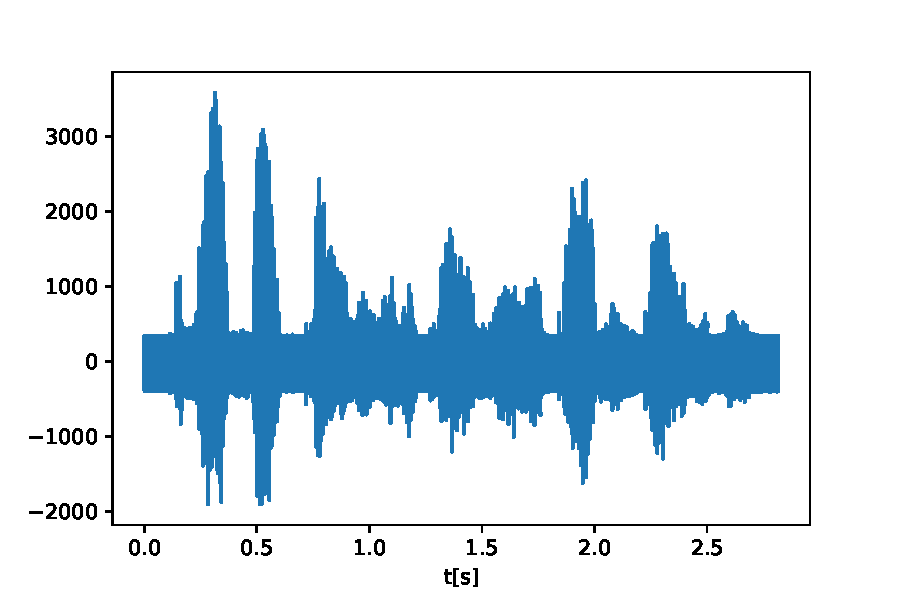
\includegraphics{img/basic.pdf}
		
		\newpage
	
	
	\section{Předzpracování a rámce}
		Signál je neprve ustředněn a normalizován.
		
		\begin{verbatim}
			data = data - data.mean()
			scale = np.abs(data).max()
			data = data / scale
		\end{verbatim}
		
		Dále je signál rozdělen na kousky o velikosti 512 pomocí metody \texttt{np.ndarray.resize}. 
		Je vytvořena prázdná matice \texttt{frames}, ve které každý sloupec bude obsahovat jeden rámec.
		Nakonec for cyklus projde všechny rámce a do každého zapíše konkatenaci dvou odpovídajících kousků.
		
		\begin{verbatim}
chunkedArray = data.reshape(numChunks, chunkSize)
frames = np.empty((numChunks-1, frameSize), dtype=float)

for i in range(numChunks-1):
    frames[i] = np.concatenate((chunkedArray[i], chunkedArray[i+1]))
		\end{verbatim}
		
		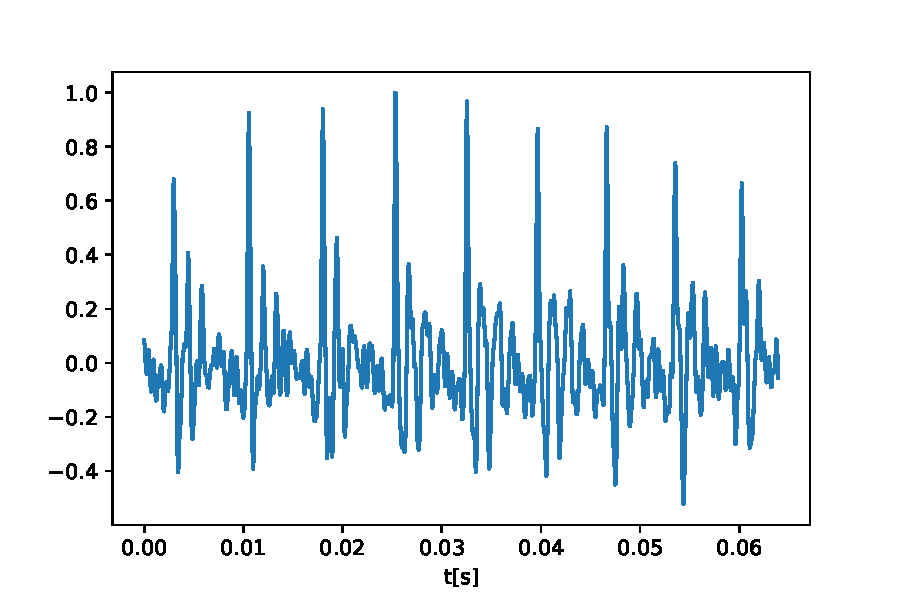
\includegraphics{img/frame.pdf}
		
		\newpage
		
	
	
	\section{DFT}
		Diskrétní fourierova transformace je implementována násobení maticí \texttt{DFT{\_}BASES}. 
		Tato matice má velikost \(1024{\times}1024\). 
		Díky tomu lze násobit s maticí \texttt{frames}, ve které jsou uloženy rámce jako sloupcové vektory.
		
		
		Je také definována funkce \texttt{DFT}, která provede maticové násobení pouze pro jeden rámec a vrátí jeho transformaci.
		
		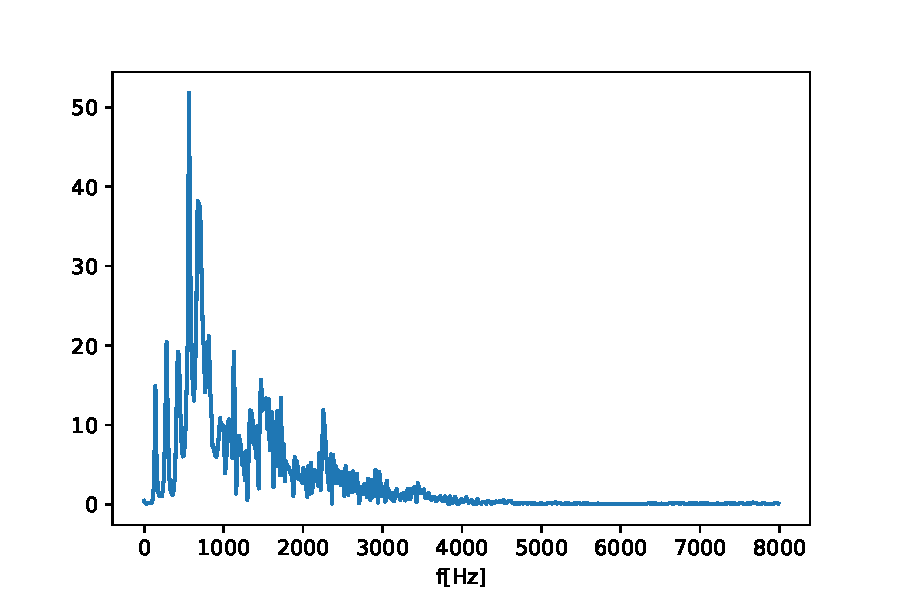
\includegraphics{img/DFT.pdf}
		
		Výstupní koeficienty funkce DFT byly porovnány s výstupy funkce \texttt{np.fft.fft}.
		Vykreslené grafy jsou na první pohled stejné. 
		Funkce \texttt{np.allclose} také potvrdila, že se výstupy shodují. 
		Tím byla implementace prohlášena za funční.
		
		\newpage
	
	
	\section{Spektrogram}
		Data pro spektrogram jsou získána fourierovou trandformací všech rámců.
		Poté je spektrogram oříznut pouze na frekvence menší než polovina vzorkovací frekvence.
		Z koeficientů DFT je udělána absolutní hodnota. 
		Jejich hodnoty jsou přepočítány na dB pro lepší dynamický rozsah při zobrazení.
		Poté je vykreslen graf funkcí \texttt{matplotlib.pyplot.imshow}.
		
		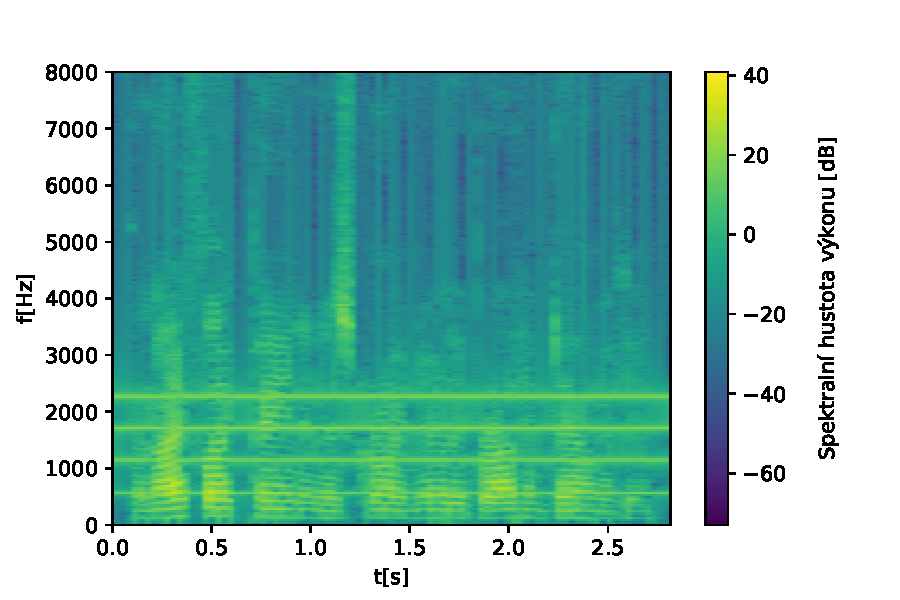
\includegraphics{img/spectrogram.pdf}
		
		\newpage
	
	
	\section{Určení rušivých frekvencí}
		Pro určení rušivých frekvencí je vhodné vybrat rámec, který obsahuje pouze je.
		Tento rámec je pomocí DFT přeměněn na koeficienty všech obsažených frekvencí.
		Tuto transformaci si opět zkrátíme do poloviny vzorkovací frekvence.
		V našem signálu jsou rušivé frekvence pouze čtyři \enquote{ostré špičky}.
		Díky tomu stačí pro jejich nalezení najít čtyři největší hodnoty v poli.
		To jde udělat metodou \texttt{ndarray.argsort}.
		Z indexů už můžeme dostat hodnoty rušivých frekvencí.
		
		\begin{verbatim}
2250.0 Hz
1687.5 Hz
1125.0 Hz
562.5 Hz
		\end{verbatim}
		
		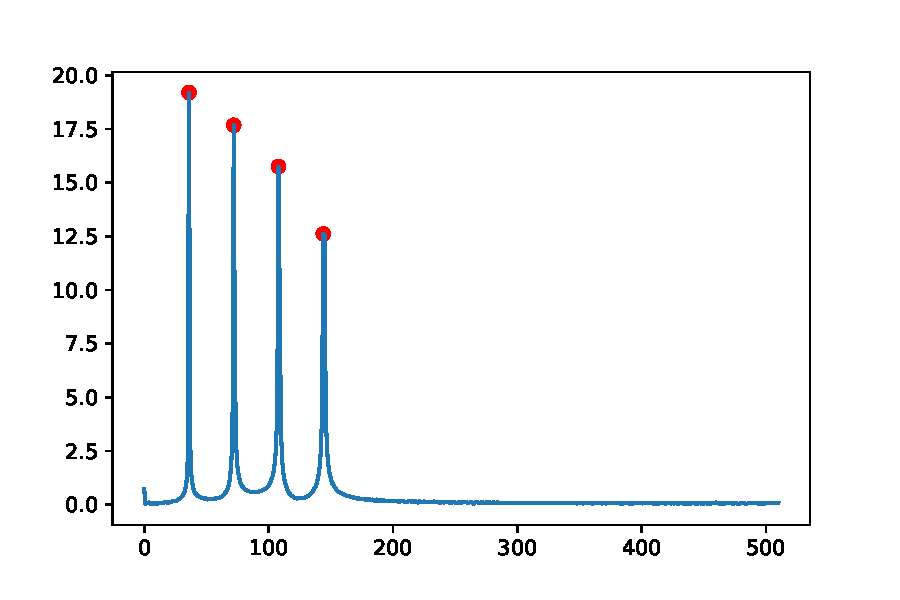
\includegraphics{img/peaks.pdf}
		
		\newpage
		
	
	
	\section{Generování signálu}
		Pro generování signálu bylo přeba inicializovat výstupní pole nulami.
		Poté bylo spuštěno generování každé frekvence pomocí for cyklu.
		Pro generovanou frekveci byla spočítána příslušná normovaná úhlová frekvence \(\omega\).
		Samotné generování proběhne na pouhém jednom řádku, kde je index v poli přeměněn na argument cosinusoidy a poté je vypočítána funkční hodnota.
		
		\begin{verbatim}
signal = np.cos(np.arange(NUM_SAMPLES) * omega)
		\end{verbatim}
		
		Tato hodnota je vydělěna počtem generovaných frekvencí a přičtena k výslednému signálu. 
		Dělení je zde z důvodu, aby rozsah výstupního signálu zůstal v uzavřeném intervalu od -1 do 1.
		
		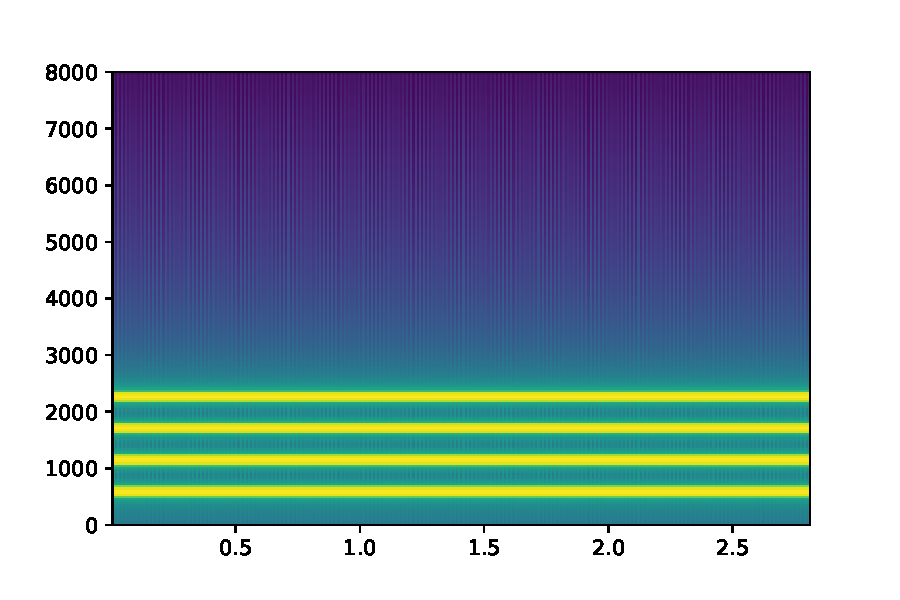
\includegraphics{img/4cos_spec.pdf}
		%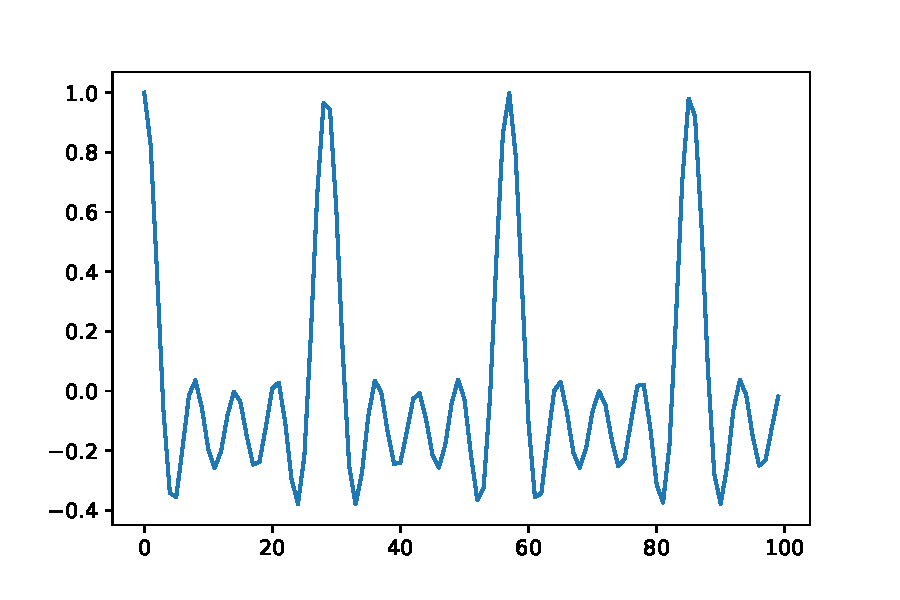
\includegraphics{img/4cos.pdf}
		
		Spektrogram vygenerovaného signálu se shoduje s rušením v zadaném signálu.
		Na poslech je také signál velmi podobný.
		
		\newpage
		
	
	
	\section{Čistící filtr}
		Jako čistící filtr jsem si vybral třetí možnost ze zadání - 4 pásmové zádrže.
		Ty jsou implementovány jako Butterworthův filtr v modulu \texttt{scipy.signal}. 
		
		Parametry zádrží jsou opět určeny podle zadání. 
		Závěrné pásmo je široké 30 Hz, s přechody širokými 50 Hz po obou stranách.
		Ripple v propustném pásmu je 3 dB a potlačení šumu -40 dB.
		
		Všechny filtry jsou po spočítání jejich koeficientů \texttt{b, a} přidány do seznamu \texttt{butter\_filters}.
		
		Nad rámec jsem také vytvořil spektrální filtr. Jeho koeficienty byly vypočítány ze spektra rámce, ve kterém je pouze hluk. Transformační funkce byla navržena tak, aby vstupu od 0 do \(\infty\) přiřazovala výstup od 1 do 0.
		
		\begin{verbatim}
spec_filter_smart = 1 / np.exp(np.abs(np.fft.fft(frames[:, 1])))
		\end{verbatim}
		
		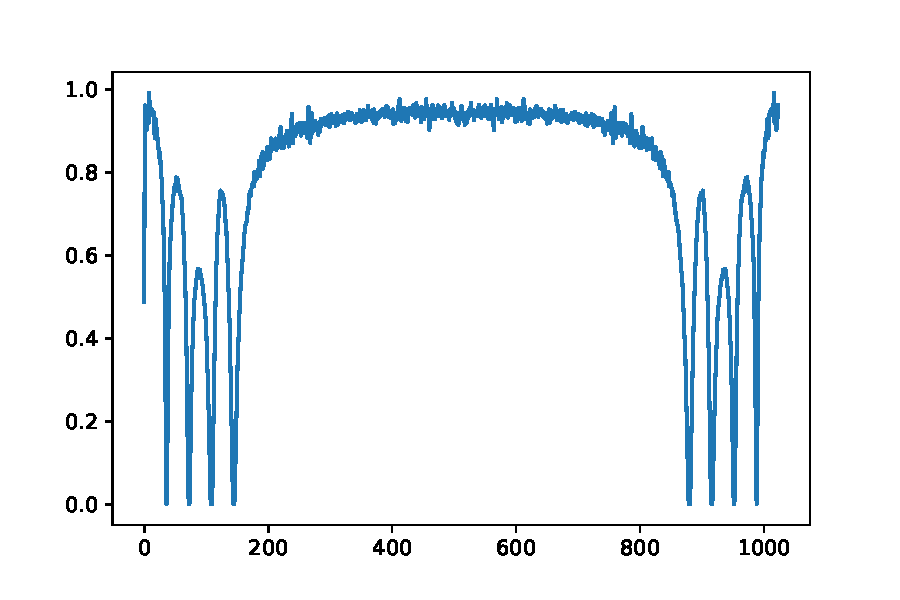
\includegraphics{img/filter_spec.pdf}
		
		\newpage
	
	\section{Nulové body a póly}
		Při vytváření Butterworthových filtrů byly také vygenerovány jejich nuly a póly.
		Ty jsou zobrazeny na jednotkové kružnici.
		
		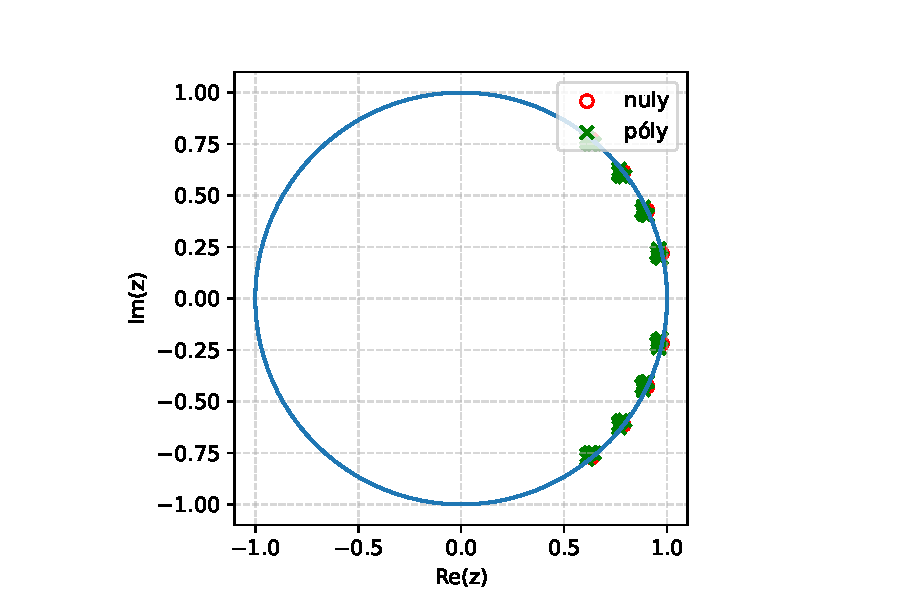
\includegraphics{img/zplane.pdf}
		
		\newpage
	
	
	\section{Frekvenční charakteristika}
		Frekvenční charakteristika Butterworthových filtrů byla získána funkcí \texttt{scipy.signal.freqz}. Ta dokáže z koeficientů \texttt{b, a} spočítat frekvenční charakteristiku.
		
		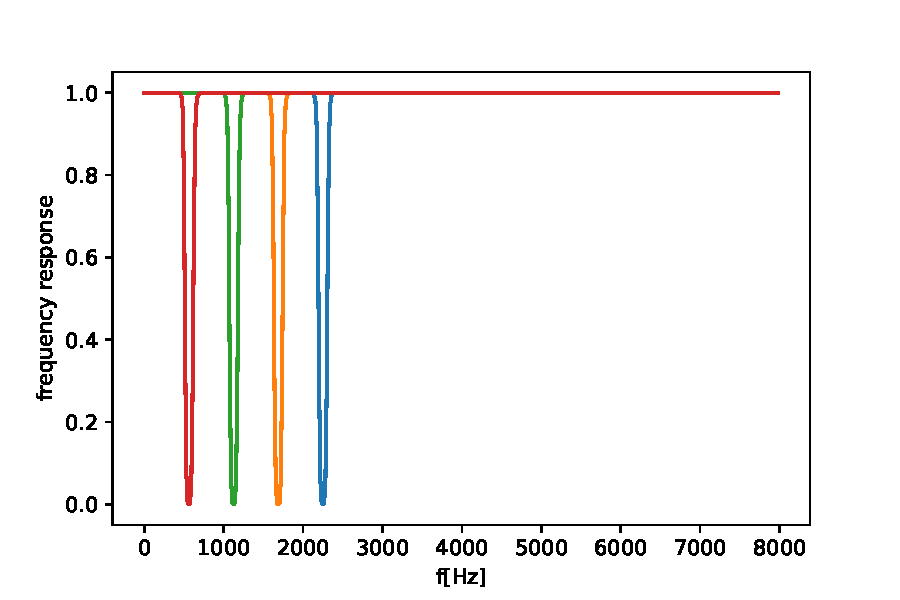
\includegraphics{img/filter_butter.pdf}
		
		\newpage
	
	
	\section{Filtrace}
	
		Filtrace pomocí Butterworthova filtru se ukázala být zcela triviální. 
		Do pole \texttt{filtered\_butter} je nejprve zkopírován původní signál.
		Poté jsou po jednom aplikovány všechny filtry. Výstupní signál je na poslech zcela čistý, nejsou slyšet žádné artefakty.
		
		\begin{verbatim}
filtered_butter = data
for b, a in butter_filters:
    filtered_butter = scipy.signal.lfilter(b, a, filtered_butter)
		\end{verbatim}
		
		Aplikace spektrálního filtru nebyla tak jednoduchá. 
		Každý rámec signálu je transformován, stejně jako při tvorbě spektrogramu.
		Poté je každý rámec vynásoben spektrálním filtrem. 
		Po inverzní fourierově transformaci jsou z rámce zachovány pouze reálné složky. Pokud bychom nyní spojili všechny rámce, náš signál by byl dvakrát delší než původní. 
		
		Okraje rámců ale mají nekvalitní signál, který by zanesl artefakty. Proto z každého rámce vyřízneme pouze prostředek. Když tyto části rámců dáme dohromady, dostáváme finální vyfiltrovaný signál. Kvalita je opět velice slušná, nejsou slyšitelné žadné artefakty.
		
		Na poslech ani nebyl mezi Butterworthovým a spektrálním filtrem žádný rozdíl. 
		Je ale velice pravděpodobné, že na \enquote{pestřejším signálu} by se rozdíl objevil.
		
		

	
		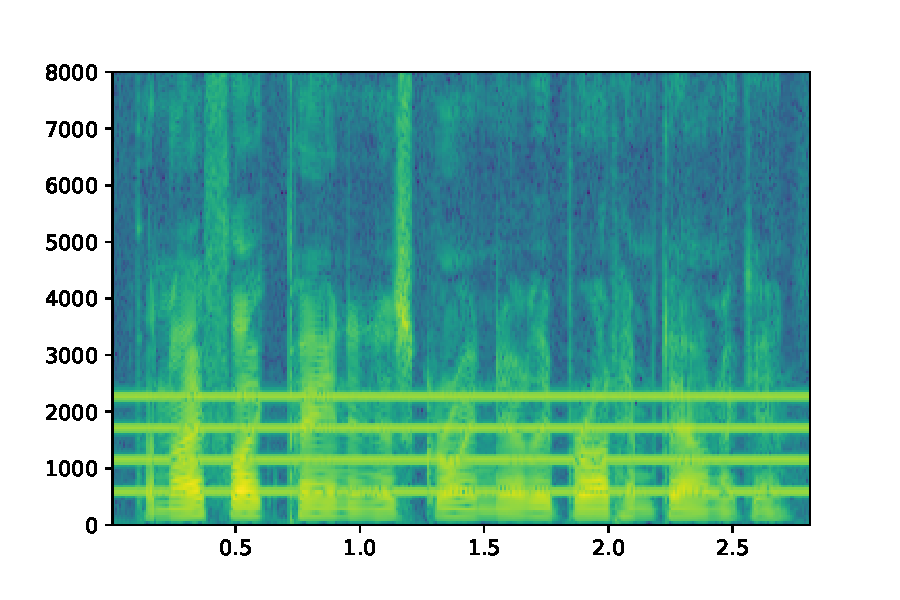
\includegraphics{img/before.pdf}
		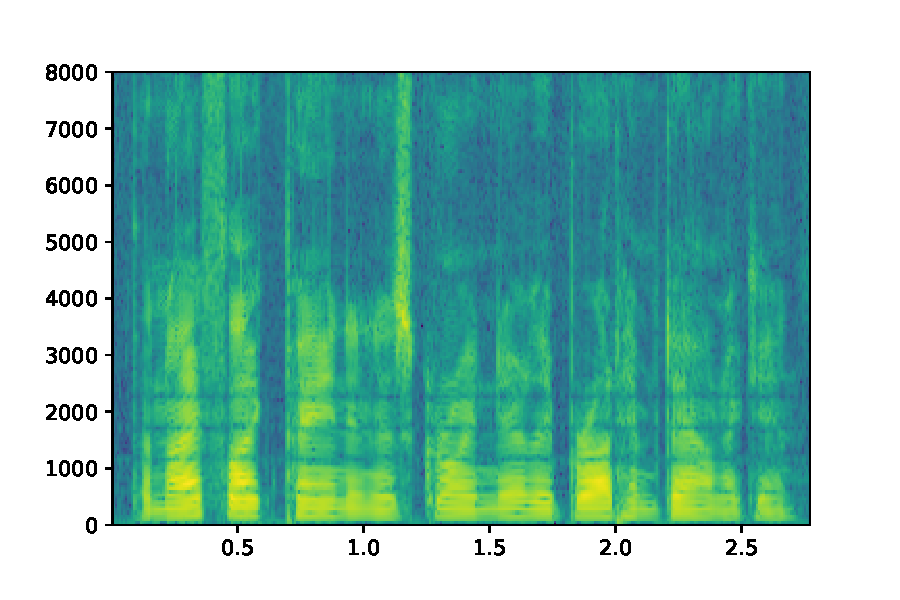
\includegraphics{img/after.pdf}
		\newpage
		
	
	
\end{document}


















































